\chapter{Compartment Models, Propagation, and Myelination}
\label{ch:compartments}

\textit{Real neurons are neither passive nor geometrically uniform. This chapter replaces analytic cables by compartment models and uses them to study propagation speed, myelination, and saltatory conduction.}

% ============================================================
\section{Multi-Compartment Models}
\label{sec:compartments}
% ============================================================

The continuous cable equation is a partial differential equation that admits analytical solutions only in special cases (passive membrane, uniform geometry). To handle realistic neurons---with nonlinear channels, varying diameters, and complex branching---we discretize the cable into a chain of compartments\index{compartmental model}.

Each compartment $n$ is a short cylinder of length $\Delta x$, assumed isopotential (uniform voltage within the compartment). Adjacent compartments are coupled by axial conductances. The voltage in compartment $n$ evolves according to
%
\begin{equation}
  \Cm\frac{\dd V_n}{\dd t} = -I_{\text{ion}}(V_n, t) + \sum_k G_{n,k}\bigl(V_k - V_n\bigr) + I_{\text{inj}}
  \label{eq:compartment}
\end{equation}
%
where $I_{\text{ion}}(V_n, t)$ is the total membrane current (which can be nonlinear---Hodgkin--Huxley channels, synaptic currents, etc.), $G_{n,k}$ is the axial conductance between compartments $n$ and $k$, and $I_{\text{inj}}$ is any injected current.

The compartmental method converts the PDE into a system of coupled ODEs---one per compartment---that can be integrated numerically. The spatial resolution must be fine enough to capture the relevant voltage gradients. A standard rule of thumb is $\Delta x \lesssim \lambda/5$; coarser discretization introduces spatial artifacts. For a typical neuron with dendrites a few hundred micrometers long and $\lambda \sim 0.5\;\text{mm}$, this means compartments of roughly $100\;\mu\text{m}$ or less.

The advantage of compartmental models is generality. Any channel type can be placed in any compartment, the geometry can be reconstructed from anatomical data, and the simulation is straightforward. The cost is that you lose the analytical insight of continuous cable theory.

% ============================================================
\section{Action Potential Propagation}
\label{sec:ap-propagation}
% ============================================================

In the passive cable, signals spread by diffusion---they decay exponentially and have no fixed velocity. Action potential propagation is qualitatively different: the spike travels as a \emph{wave} that regenerates itself at each point along the axon, maintaining constant amplitude and shape.

The mechanism is local positive feedback. At the wavefront, the voltage is rising, which opens sodium channels in the adjacent (resting) membrane. The inward sodium current depolarizes that region, opening more channels, and the wavefront advances. Behind the wavefront, the membrane is in its refractory period (sodium inactivated, potassium still open), so the wave cannot travel backward.

\subsection{Propagation speed in unmyelinated axons}

The speed of the action potential depends on how quickly the wavefront can depolarize the next stretch of membrane. The relevant timescale is $\taum$ (how fast the membrane charges) and the relevant length scale is $\lambda$ (how far ahead the axial current reaches). Dimensional analysis gives

\begin{keyequation}[AP Propagation Speed (Unmyelinated)]
\begin{equation}
  v_{\text{AP}} \approx \frac{2\lambda}{\taum} \propto \sqrt{a}
  \label{eq:ap-speed}
\end{equation}
\tcblower
$\lambda \propto \sqrt{a}$: length constant, \quad
$\taum = r_m c_m$: membrane time constant (independent of $a$). \\[4pt]
Speed scales as $\sqrt{a}$: doubling the speed requires quadrupling the radius.
\end{keyequation}

\noindent For typical unmyelinated axon parameters, this gives $v_{\text{AP}} \sim 0.1$--$1\;\text{m/s}$. The squid giant axon achieves high speed ($\sim 25\;\text{m/s}$) by having an enormous radius ($\sim 0.5\;\text{mm}$). This brute-force strategy is metabolically expensive and takes up a lot of space. Vertebrates use a different solution: myelination.

\subsection{Wave properties}

Action potential waves have several notable properties. They travel in both directions from the initiation site (orthodromic and antidromic propagation). Two colliding waves annihilate each other, because the membrane behind each wavefront is refractory. Waves do not reflect from sealed ends or branch points (though they can fail to propagate past a branch point if the impedance load of the daughters is too large).

% ============================================================
\section{Myelination}
\label{sec:myelination}
% ============================================================

Myelin\index{myelination} is a lipid-rich insulating sheath wrapped around axons by glial cells (oligodendrocytes in the central nervous system, Schwann cells in the peripheral nervous system). The myelin is interrupted at regular intervals by \emph{nodes of Ranvier}\index{nodes of Ranvier}, where the axon membrane is exposed and densely packed with sodium channels.

Myelination changes two membrane parameters. The insulating wraps increase the effective membrane resistance $r_m^*$ (less leakage through the sheath) and decrease the effective membrane capacitance $c_m^*$ (the myelin acts as a series capacitance). For a sheath with inner radius $a_1$ (the axon) and outer radius $a_2$ (including myelin):
%
\begin{equation}
  r_m^* = r_m\,\frac{a_1}{d}\,\ln\!\Bigl(\frac{a_2}{a_1}\Bigr), \qquad
  c_m^* = c_m\,\frac{d}{a_1\,\ln(a_2/a_1)}
  \label{eq:myelin-params}
\end{equation}
%
where $d$ is the membrane thickness. The product $r_m^* c_m^* \approx r_m c_m$, so the time constant is approximately unchanged. But the length constant increases dramatically: $\lambda^* \propto \sqrt{r_m^*} \gg \lambda$.

\subsection{Reduced myelinated-cable scaling}

For an internode segment (no active regeneration), the cable equation becomes
%
\begin{equation}
  r_m^* c_m^*\,\frac{\partial v}{\partial t}
  =
  \frac{r_m^* a_1}{2r_L}\,\frac{\partial^2 v}{\partial x^2}
  - v.
  \label{eq:myelin-cable}
\end{equation}
%
On internodal timescales where longitudinal spread dominates local leak, the $-v$ term is subleading, giving an effective diffusion equation:
%
\begin{equation}
  \frac{\partial v}{\partial t} = D_* \frac{\partial^2 v}{\partial x^2},
  \qquad
  D_*=\frac{a_1}{2r_L c_m^*}
  =\frac{a_1^2\ln(a_2/a_1)}{2r_L c_m d}.
  \label{eq:myelin-diffusion}
\end{equation}
%
Thus, geometry controls the dominant propagation scale through the factor
$a_1^2\ln(a_2/a_1)$.

At fixed outer radius $a_2$, maximizing this factor yields
$a_1/a_2=1/\sqrt{e}$, exactly the optimum in \cref{eq:optimal-ratio}. This provides a compact derivation of why the same ratio emerges from conduction-speed and electrotonic-length arguments.

\subsection{Saltatory conduction}

Conduction in myelinated axons is \emph{saltatory}\index{saltatory conduction}: the action potential ``jumps'' from node to node. At each node, voltage-gated sodium channels regenerate the spike. Between nodes, current spreads passively through the myelinated internode with minimal leakage and minimal capacitive loading. The result is much faster conduction.

The key change is that the propagation speed now scales linearly with the outer radius rather than as its square root:
%
\begin{equation}
  v_{\text{AP}}^{\text{myel}} \propto a_2
  \label{eq:myelin-speed}
\end{equation}
%
This is a dramatic improvement. A myelinated axon of $10\;\mu\text{m}$ diameter can conduct at $50$--$100\;\text{m/s}$, comparable to the squid giant axon at $500\;\mu\text{m}$ diameter. Myelination achieves the same speed with $\sim 2500$ times less cross-sectional area.

\subsection{Empirical anchoring}

Peripheral-nerve measurements (e.g., cat fibers) show an approximately linear conduction-velocity trend with fiber diameter over a broad range, consistent with the scaling in \cref{eq:myelin-speed}. A practical rule of thumb is that each additional micrometer of myelinated fiber diameter contributes several meters per second of conduction speed.

The linear trend is not exact---node spacing, temperature, and channel density also matter---but the first-order dependence on outer diameter is robust and is one of the clearest biophysical signatures of saltatory conduction.

Computationally, this empirical relation explains why long-range pathways can simultaneously be fast and compact: conduction delay can be tuned by modest anatomical changes without requiring giant axons.

\subsection{Optimal myelin thickness}

How thick should the myelin be? Thicker myelin increases $r_m^*$ and $\lambda^*$, but it also increases the outer radius $a_2$, which takes up space. There is an optimum ratio of inner to outer radius that maximizes the length constant for a fixed outer diameter:
%
\begin{equation}
  \frac{a_1}{a_2} = \frac{1}{\sqrt{e}} \approx 0.6
  \label{eq:optimal-ratio}
\end{equation}
%
This means the axon should occupy about $60\%$ of the total fiber diameter, with $40\%$ being myelin. Remarkably, measurements of real myelinated axons consistently find ratios of $0.6$--$0.7$, close to the theoretical optimum. Biology has found the solution predicted by the mathematics.

\begin{figure}[h]
\centering
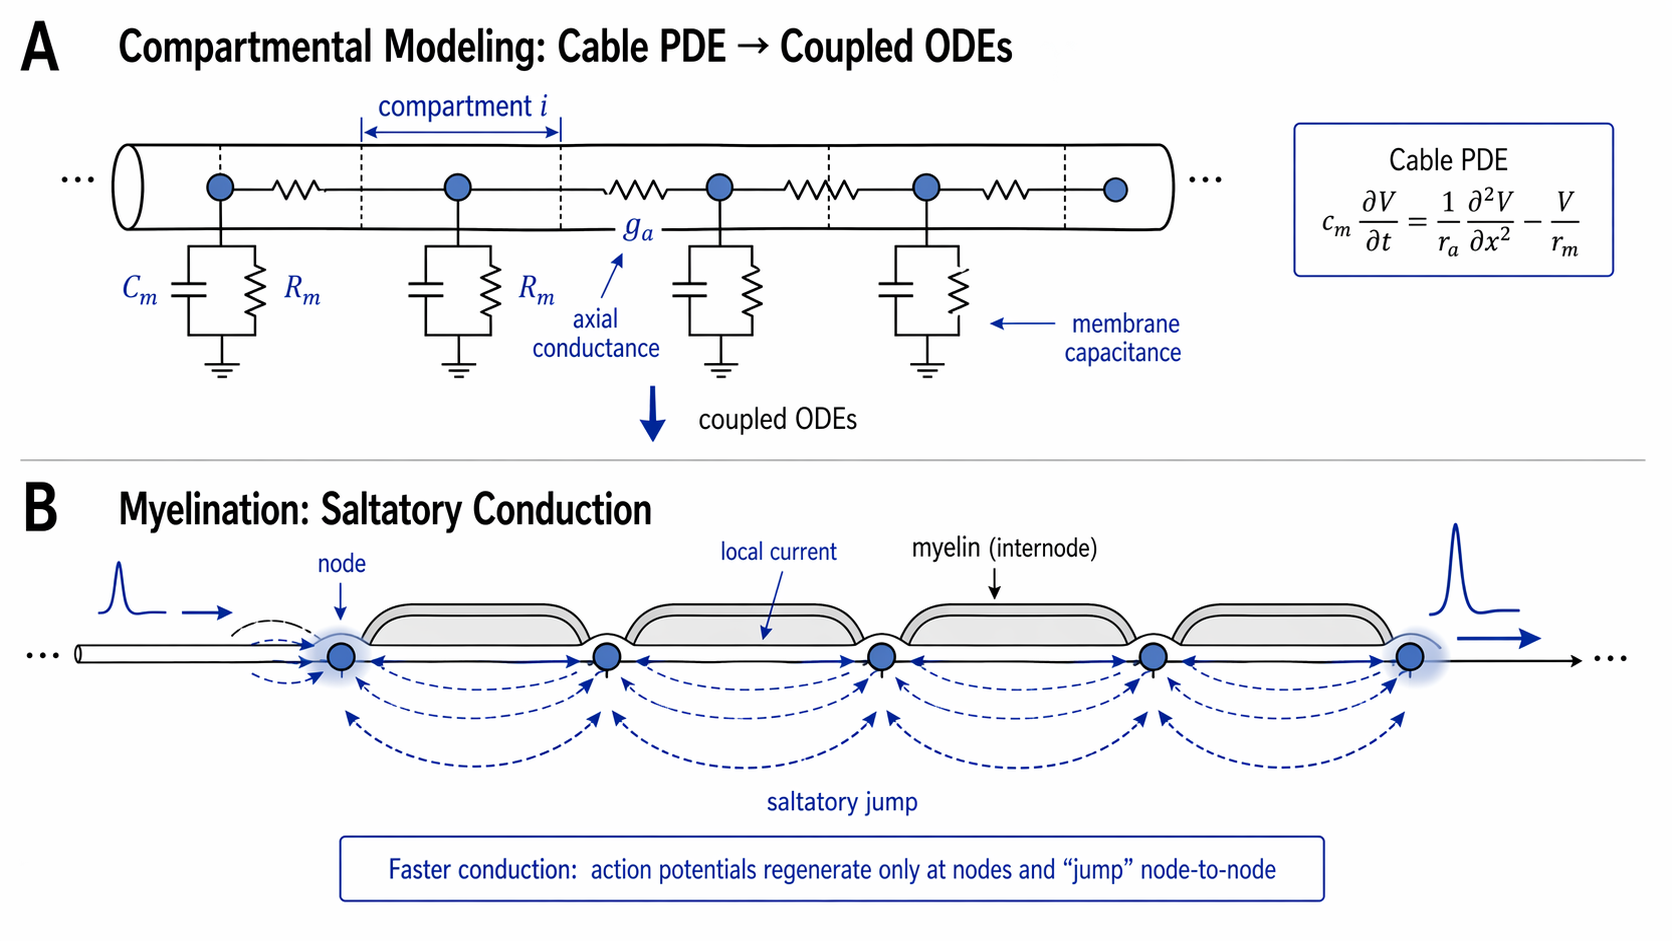
\includegraphics[width=\textwidth]{figures/mns-compartment-myelination.png}
\caption{Compartmental and myelinated models. Spatial discretization turns the cable PDE into coupled ODEs, while myelin increases effective spread between active nodes so spikes regenerate saltatorily.}
\label{fig:compartment-myelination}
\end{figure}


\begin{chaptersummary}

\begin{center}
\renewcommand{\arraystretch}{1.6}
\begin{tabularx}{\textwidth}{@{}l X X@{}}
  \toprule
  \textbf{Concept} & \textbf{Equation} & \textbf{Key Insight} \\
  \midrule
  Compartmental model &
  $\Cm\dot{V}_n = -I_{\text{ion}} + \sum G_{n,k}(V_k - V_n)$ &
  Discretize cable for numerical simulation \\
  %
  AP speed (unmyelinated) &
  $v \approx 2\lambda/\taum \propto \sqrt{a}$ &
  Square-root scaling: slow without myelin \\
  %
  Myelin effect &
  $r_m^* \uparrow$, $c_m^* \downarrow$, $\lambda^* \uparrow$ &
  Less leakage, less capacitance \\
  %
  Reduced internode dynamics &
  $\partial_t v = D_*\,\partial_x^2 v$ &
  Geometry-controlled rapid passive spread between nodes \\
  %
  Saltatory conduction &
  Node-to-node regeneration &
  Speed $\propto a_2$ (linear scaling) \\
  %
  Optimal ratio &
  $a_1/a_2 = 1/\sqrt{e} \approx 0.6$ &
  Biology matches the theoretical optimum \\
  \bottomrule
\end{tabularx}
\end{center}

\end{chaptersummary}

\begin{conceptquestions}
  \item The compartmental model converts the cable PDE into a system of coupled ODEs. What is lost in this discretization? What determines how fine the spatial grid must be?

  \item In a compartmental model, what determines how fine the spatial discretization must be? What goes wrong if $\Delta x$ is too large compared to $\lambda$?

  \item Compare the compartmental model to the equivalent cylinder approach from \cref{ch:cable-branching}. What are the advantages and limitations of each?

  \item Action potential propagation is fundamentally different from passive spread: the spike maintains its amplitude as it travels. Explain the mechanism of regeneration at each point along the axon.

  \item Why does the action potential travel in only one direction under normal physiological conditions, even though the physics would allow bidirectional propagation? What prevents backward propagation?

  \item Action potential speed in unmyelinated axons scales as $\sqrt{a}$, but in myelinated axons it scales as $a$. Explain the physical reason for this difference.

  \item The squid giant axon achieves fast conduction by having a very large radius ($\sim 0.5\;\text{mm}$). A myelinated vertebrate axon of only $10\;\mu\text{m}$ diameter conducts at comparable speed. Calculate roughly how much cross-sectional area the myelinated solution saves.

  \item Myelination increases $r_m^*$ and decreases $c_m^*$, but the product $r_m^* c_m^*$ stays roughly constant. Why does the conduction speed increase if the time constant does not change?

  \item In saltatory conduction, the action potential ``jumps'' from node to node. What happens at each node? What happens in the internode? Why is this faster than continuous regeneration?

  \item The optimal ratio $a_1/a_2 \approx 0.6$ maximizes the length constant for a fixed outer diameter. What happens if the myelin is too thin (ratio near 1)? What if it is too thick (ratio near 0)?

  \item The optimal ratio $a_1/a_2 = 1/\sqrt{e}$ is derived from maximizing $\lambda^*$ at fixed outer radius. Measurements of real axons give ratios of $0.6$--$0.7$. What does this agreement between theory and biology suggest about evolutionary optimization?

  \item Two action potential waves traveling toward each other on the same axon annihilate when they meet. Why? What is the state of the membrane at the collision point?

  \item Demyelinating diseases like multiple sclerosis strip myelin from axons. Using what you know about the effects of myelination on $r_m^*$, $c_m^*$, and $\lambda^*$, predict the consequences for conduction speed. At what point would conduction fail entirely?
\end{conceptquestions}
